\section{Общие соображения об управлении сложными системами. Декомпозиция траекторной задачи и задачи стабилизации применительно к многозвенному манипулятору.}

С увеличением сложности объекта управления более успешными становятся сложные, многокаскадные системы управления. Попытка внедрения функционала прохождения траектории или обхода препятствий непосредственно в алгоритм системы стабилизации или системы задания координат, хотя и может претендовать на достижения неких оптимальных показателей, представляется сомнительной с инженерной точки зрения, поскольку приводит к сильной связности алгоритмов управления, неочевидности поведения системы, требует трудоёмкой аналитической переработки при внесении изменений в функционал управления, повышает требования к квалификации работников технического сопровождения.

Разделив задачу управления на несколько слабо связанных задач, можно использовать каждое из них для введения уставки следующей. Так мы можем задавшись некоторыми ограничениями на динамические возможностями нашей системы, построить решение задачи траекторного управления достаточной точности, учитывающее обход препятствий всеми звеньями кинематической цепи без необходимости просчета временных функции кинематических координат $q_i(t)$. 

С другой стороны мы обеспечиваем решение задачи координатного управления, чтобы все уставки $P_i(t)$ выданные для каждого момента времени траекторным алгоритмом выполнялись с необходимой точностью.

Такое разбиение позволяет координатному решателю не заботиться о геометрических ограничениях ввиду того, что они учтены траекторным решателем, а траекторный решатель может расчитывать управление траектории в удобных для этой задачи координатах, поскольку не связан необходимостью физического управления изделием.   

\begin{center}
  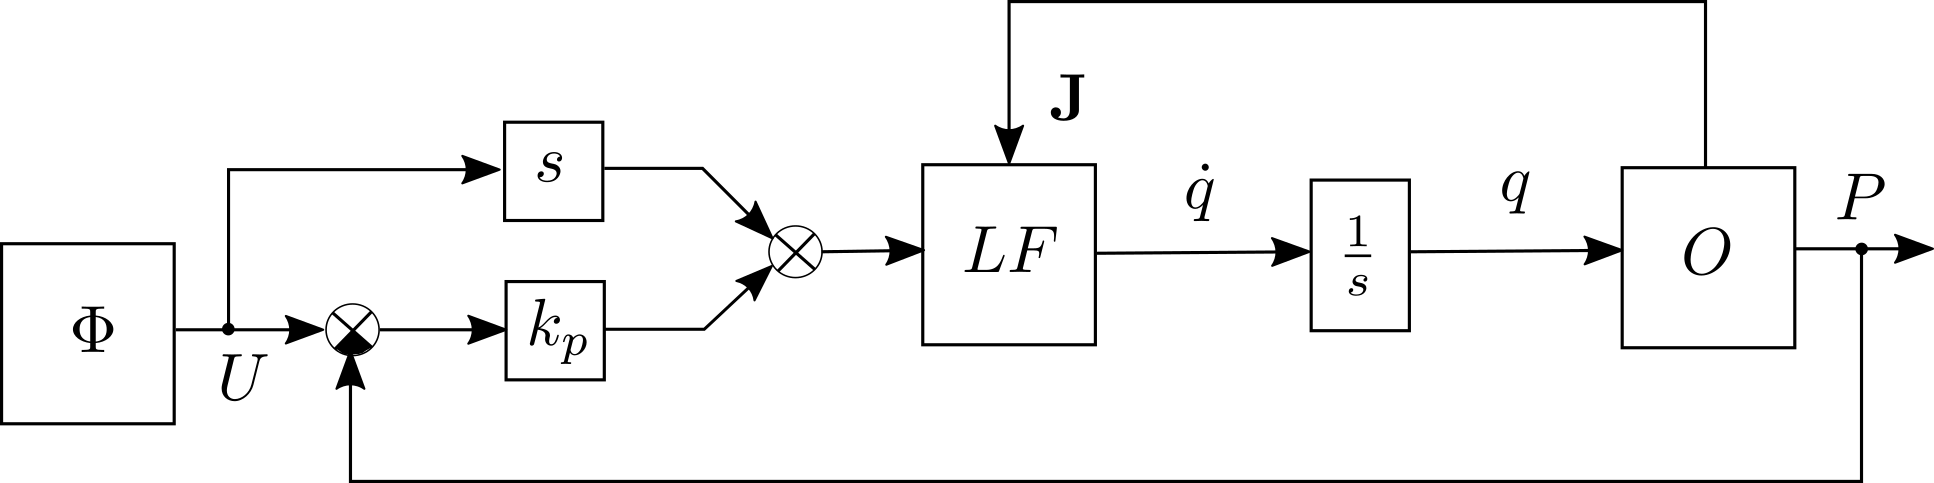
\includegraphics[width=\textwidth,height=\textheight,keepaspectratio]{ctrsyst.png}
  \captionof{figure}{Структурная схема полученной системы.}
  \label{}
\end{center}